\documentclass[12pt, titlepage]{article}
\usepackage[utf8]{inputenc}
\usepackage[spanish]{babel}
\usepackage[letterpaper, margin=2.5cm]{geometry}
\usepackage{lipsum}
%\usepackage[nottoc,numbib]{tocbibind}
\usepackage{float}
\usepackage{amsmath}
\usepackage{url}
\usepackage{graphicx} 

\usepackage{listings}
\usepackage{color}
\definecolor{dkgreen}{rgb}{0,0.6,0}
\definecolor{gray}{rgb}{0.5,0.5,0.5}
\definecolor{mauve}{RGB}{253,151,31}

\lstset{frame=tb,
	aboveskip=3mm,
	belowskip=3mm,
	showstringspaces=false,
	columns=flexible,
	basicstyle={\small\ttfamily},
	numbers=none,
	numberstyle=\tiny\color{gray},
	keywordstyle=\color{blue},
	commentstyle=\color{dkgreen},
	stringstyle=\color{mauve},
	breaklines=true,
	breakatwhitespace=true,
	tabsize=3
}

\title{Reporte del primer parcial}
\author{Carlos Tonatihu Barrera Pérez \\ Profesor: Genaro Juárez Martínez \\ Teoría Computacional \\ Grupo: 2CM4 }
\date{10 de septiembre de 2016}
\begin{document}
	\maketitle
	\tableofcontents
	
		\section{Alfabeto}
	\subsection{Descripción del problema}
	El objetivo de esta practica es el generar las potencias del alfabeto binario $ \sum = \lbrace 0, 1 \rbrace $ desde $k=0$ hasta un $k$ seleccionado con un máximo de $k=1000$, para después guardar en un archivo todas las cadenas que se pudieron formar bajo estas condiciones, es decir: 
	\[{\sum}^{+} = {\sum}^{0}\cup{\sum}^{1}\cup{\sum}^{2}\cup\cdots\cup{\sum}^{1000}\]
	Es importante señalar que este conjunto solo es un subconjunto de $ {\sum}^{*} $ que representa todas las cadenas que se pueden formar con este alfabeto binario.
	El programa cuenta con modo manual (el usuario ingresa un $k$) y automático (genera su propio $k$).
	\subsection{Código}
	El código del programa fue realizado en C.
	\\Archivo: albafeto.h
	\begin{lstlisting}[language=C]
	//albafeto.h
	#ifndef __ALFABETO__
	#define __ALFABETO__
	
	#include <stdio.h>
	#include <stdlib.h>
	#include <time.h>
	
	static const int CONTINUAR = 1;
	int iniciar();
	int abrir_archivo(FILE **);
	int generar_palabras();
	
	#endif
	\end{lstlisting}
	Archivo: alfabeto.c
	\lstset{language=C}
	\begin{lstlisting}
	//alfabeto.c
	#include "alfabeto.h"
	
	int generar_palabras(int potencia_k) {
		FILE *archivo = NULL;
		int long_cadena;
		int i;
		int posicion;
		int *cadena_aux = NULL;
		
		abrir_archivo(&archivo);
		fputs("S = {e", archivo);
		
		for (long_cadena = 1; long_cadena <= potencia_k; long_cadena++) {
			cadena_aux = (int*) calloc(long_cadena, sizeof(int));
			if(cadena_aux == NULL) {
				printf("%s\n", "Error en el calloc");
				exit(0);
			}
			while(CONTINUAR) {
				fputc(',', archivo);
				for(i = 0; i < long_cadena; i++) {
					fputc(cadena_aux[i] + '0', archivo);
				}
				for(posicion = 0; posicion < long_cadena; posicion++) {
					cadena_aux[posicion] += 1;
					if(cadena_aux[posicion] > 1) {
						cadena_aux[posicion] = 0;
					} else {
						break;
					}
				}
				if(posicion >= long_cadena) {
					free(cadena_aux);
					break;
				}
			}
			printf("Va en 2^%d\n", long_cadena);
		}
		
		fputs("}", archivo);
		fclose(archivo);
		return 1;
	}
	
	int abrir_archivo(FILE **archivo) {
		*archivo = fopen("palabras.txt", "w");
		if (*archivo == NULL) {
			printf("%s\n", "No se pudo abrir");
			exit(0);
		}
		return 1;
	}
	
	\end{lstlisting}
	Archivo: main.c
	\begin{lstlisting}[language=C]
	//albafeto.h
	#include "main.c"
	
	int iniciar();
	int menu();
	int menu_continuar();
	int random_potencia_k();
	
	int main(int argc, char const *argv[]) {
		printf("%s\n", "***************Alfabeto****************");
		iniciar();
		return 0;
	}
	
	int iniciar() {
		srand(time(NULL));
		int continuar = 1;
		int potencia_k = 1;
		int manual = 1;
		while(continuar) {
			manual = menu();
			if (manual == 1) {
				printf("%s\n", "Ingresa el valor de k: ");
				scanf("%d", &potencia_k);
			} else if (manual == 2) {
				potencia_k = random_potencia_k();
			} else {
				break;
			}
			printf("El valor de k es: %d\n", potencia_k);
			generar_palabras(potencia_k);
			printf("%s\n", "Cadenas guardadas en el archivo palabras.txt");
			continuar = menu_continuar();
		}
		printf("\n%s\n", "Saliendo...");
		return 1;
	}
	
	int menu_continuar() {
		int opcion;
		printf("Intentar otra vez?\nSi = 1 NO = 0\n");
		scanf(" %d", &opcion);
		return opcion;
	}
	
	int menu() {
		int opcion;
		printf("Que quieres hacer?\n1.-Manual\n2.-Automatico\n3.-Salir\n");
		scanf(" %d", &opcion);
		return opcion;
	}
	
	int random_potencia_k() {
		//numero = rand () % (N-M+1) + M;
		// Cambiar el valor del random k a 1000
		int potencia_k = 1 + rand() % (1000 + 1 - 1);
		return potencia_k;
	}
	\end{lstlisting}
	\subsection{Pruebas}
	Las pruebas están divididas en modo automático y manual, en ambos dada una k se generan todas las cadenas de longitud 1 hasta $k$.
	\\\\
	{\large Modo automático.}
	\begin{figure}[H]
		\begin{center}
			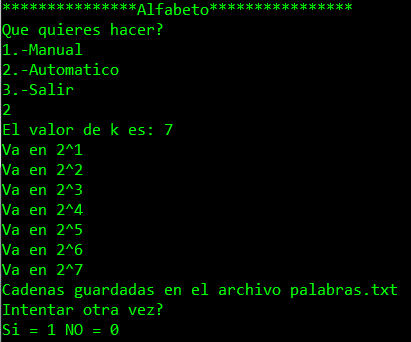
\includegraphics[width=7cm, height=7cm]{img/automatico-alfabeto.png}
			\caption{Alfabeto con k = 7.}
			\label{fig:alfabeto1}
		\end{center}
	\end{figure}
	\begin{figure}[H]
		\begin{center}
			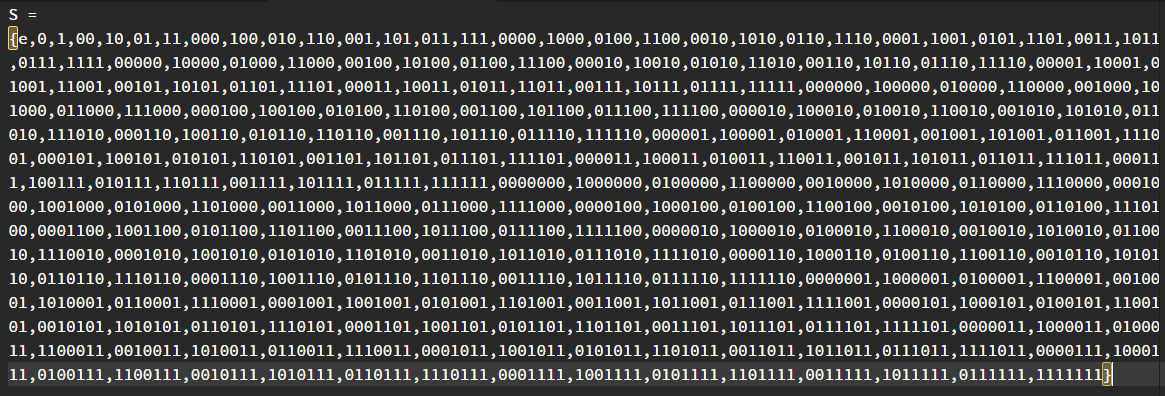
\includegraphics[width=\linewidth, height=8cm]{img/automatico-alfabeto-salida.png}
			\caption{Archivo generado.}
			\label{fig:alfabeto2}
		\end{center}
	\end{figure}
	{\large Modo manual.}
	\begin{figure}[H]
		\begin{center}
			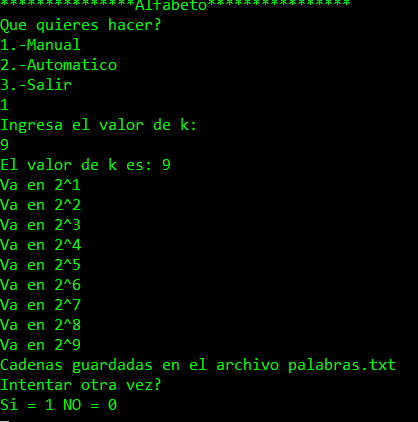
\includegraphics[width=7cm, height=7cm]{img/manual-alfabeto.png}
			\caption{Alfabeto con k = 9.}
			\label{fig:alfabeto3}
		\end{center}
	\end{figure}
	\begin{figure}[H]
		\begin{center}
			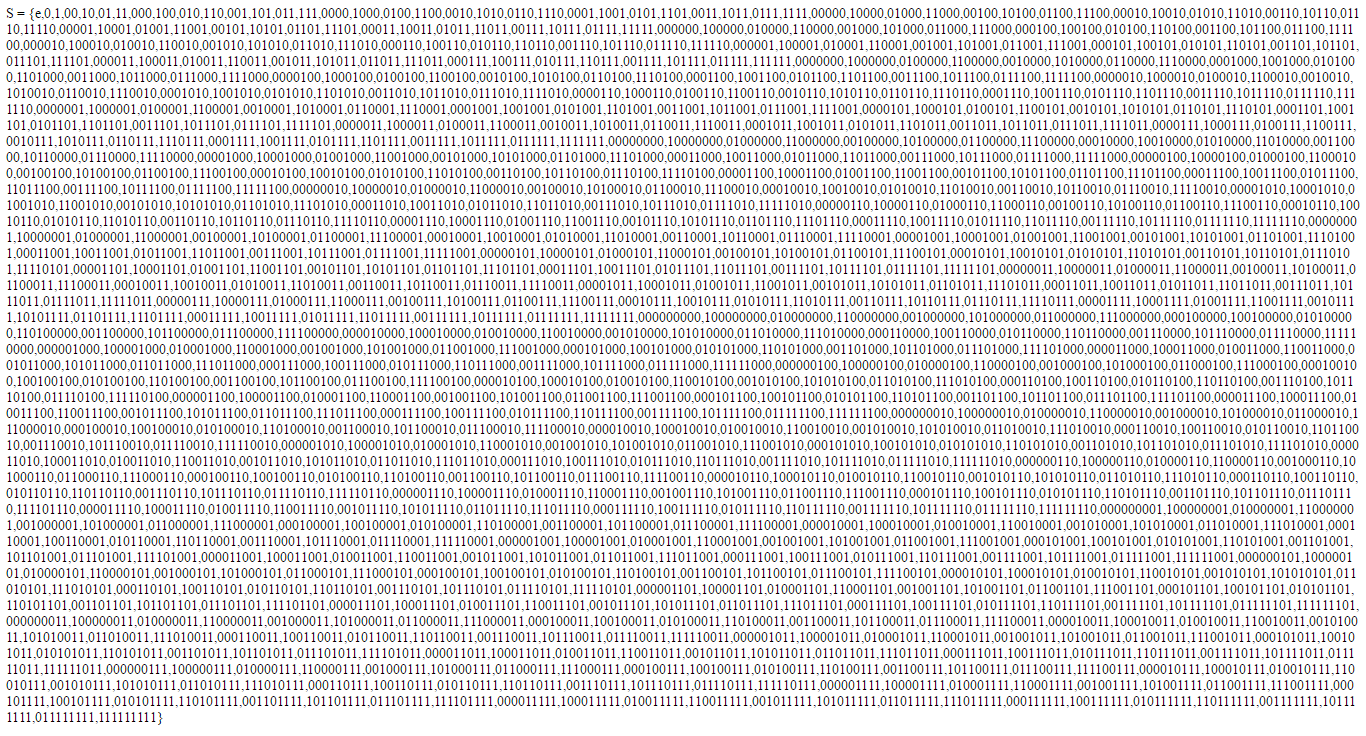
\includegraphics[width=\linewidth, height=12cm]{img/manual-alfabeto-salida.png}
			\caption{Archivo generado.}
			\label{fig:alfabeto4}
		\end{center}
	\end{figure}
	\section{Números primos}
	\subsection{Descripción del problema}
	Desarrollar un programa que encuentre todos los números primos en el intervalo $0 \leq n \leq 1000$ imprimirlos en pantalla junto con su representación en binario ademas de contar la cantidad de ceros y unos en dicho numero, finalmente guarda los números primos en su forma binaria en un archivo txt.
	Cuenta con modo manual (el usuario ingresa un numero n) y automático (el programa utiliza un $n$ aleatorio).
	\subsection{Código}
	El código del programa fue realizado en Python 3.5.
	\\
	Archivo: primos.py
		\begin{lstlisting}[language=Python]
		# primos.py
		# -*- coding: utf-8 -*-
		from __future__ import print_function
		import math, random
		
		separador = '*'*50
		
		def iniciar():
		maximo = 1
		continuar = True
		
		while continuar:
			archivo = open('primos.txt', 'w')
			lista_primos = []
			lista_binarios = []
			manual = imprimir_menu()
			if manual == 1:
				maximo = int(input("Escribe un numero entre 1 y 1000 "))
			elif manual == 2:
				maximo = random_maximo()
			else:
				break
			print("El limite es: ", maximo)
			lista_primos = calcular_primos(maximo)
			lista_binarios = conversion_binaria(lista_primos, archivo)
			print(lista_primos)
			print('*'*50)
			print(lista_binarios)
			contar_repeticiones(lista_binarios, lista_primos)
			print('Numeros primos en binarios guardados en primos.txt')
			archivo.close()
			opcion = input("Reintentar s/n: ")
			if opcion.lower() != 's':
				continuar = False
			
		print('Saliendo...')
		
		def random_maximo():
			return random.randint(1, 1000)
		
		def calcular_primos(maximo):
			lista_primos = []
			es_primo = False
			if maximo < 2:
				es_primo = False
			else:
				lista_primos.append(2)
				for numero_actual in range(2, maximo + 1):
					raiz = math.sqrt(numero_actual)
					if raiz == round(raiz):
						es_primo = False
					else:
						for num in lista_primos:
							if num > math.ceil(raiz):
								break
							if numero_actual % num == 0:
								es_primo = False
								break
							else:
								es_primo = True
						if es_primo:
							lista_primos.append(numero_actual)
			return lista_primos
		
		def imprimir_menu():
			print('\n\n%sMenu%s' % (separador, separador))
			print("""
			1.- Manual
			2.- Automatico
			3.- Salir
			""")
			try:
				opcion = int(input("Selecciona una opcion valida: "))
				return opcion
			except Exception as e:
				print('Error ', e)
				return 0
		
		def conversion_binaria(lista_primos, archivo):
			lista_binarios = []
			archivo.write('{')
			for numero in lista_primos:
				lista_binarios.append(bin(numero)[2:])
				archivo.write('%s,' % bin(numero)[2:])
			
			archivo.write('}')
			return lista_binarios
		
		def contar_repeticiones(lista_binarios, lista_primos):
			total = []
			i = 0
			for valor in lista_binarios:
				ceros, unos = 0, 0
				for digito in valor:
					if digito == '0':
						ceros += 1
					else:
						unos += 1
				total.append({'Numero': lista_primos[i], 'Ceros': ceros, 'Unos': unos})
				i += 1
			for numero in total:
				print('Numero: %s No. Ceros: %s No. Unos: %s' % (numero['Numero'], numero['Ceros'], numero['Unos']))
			
		iniciar()
		
		\end{lstlisting}
	\subsection{Pruebas}
	Las pruebas están divididas en modo automático y manual.
	\\{\large Modo automático.}
		\begin{figure}[H]
			\begin{center}
				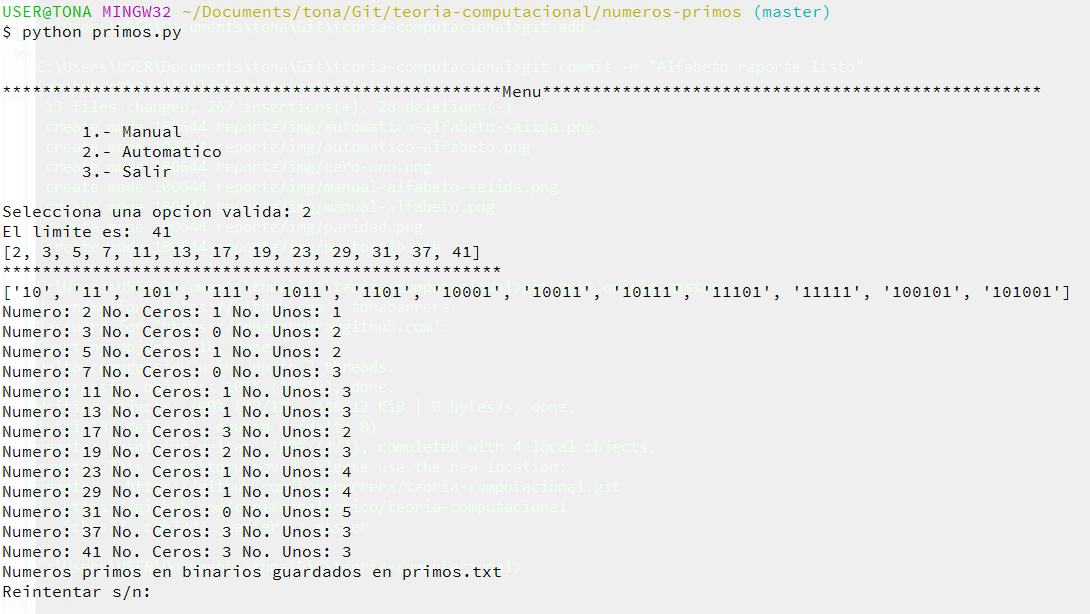
\includegraphics[width=\linewidth, height=6cm]{img/primos-automatico.png}
				\caption{Modo automático n=41.}
				\label{fig:primos1}
			\end{center}
		\end{figure}
			\begin{figure}[H]
				\begin{center}
					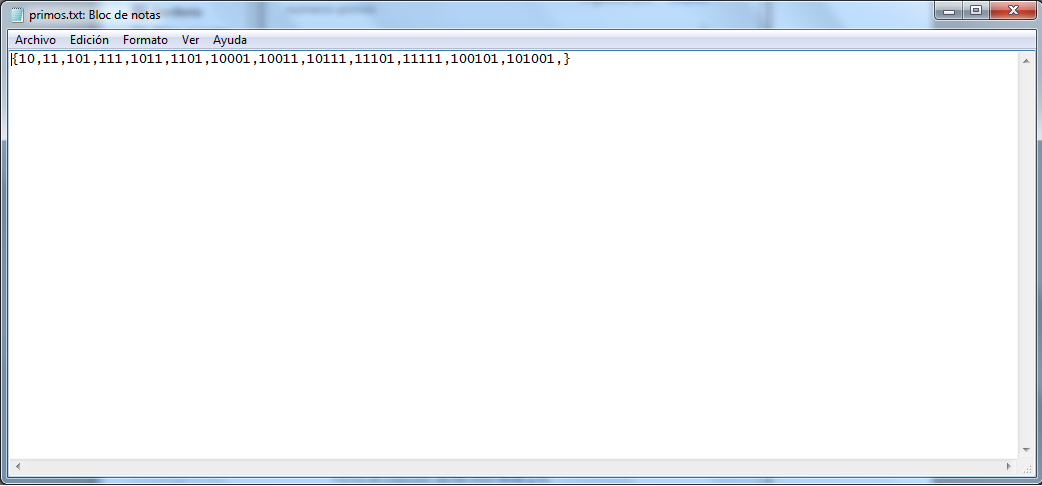
\includegraphics[width=\linewidth, height=7cm]{img/primos-automatico-salida.png}
					\caption{Números primos en binario en el archivo.}
					\label{fig:primos2}
				\end{center}
			\end{figure}
	{\large Modo manual.}
		\begin{figure}[H]
			\begin{center}
				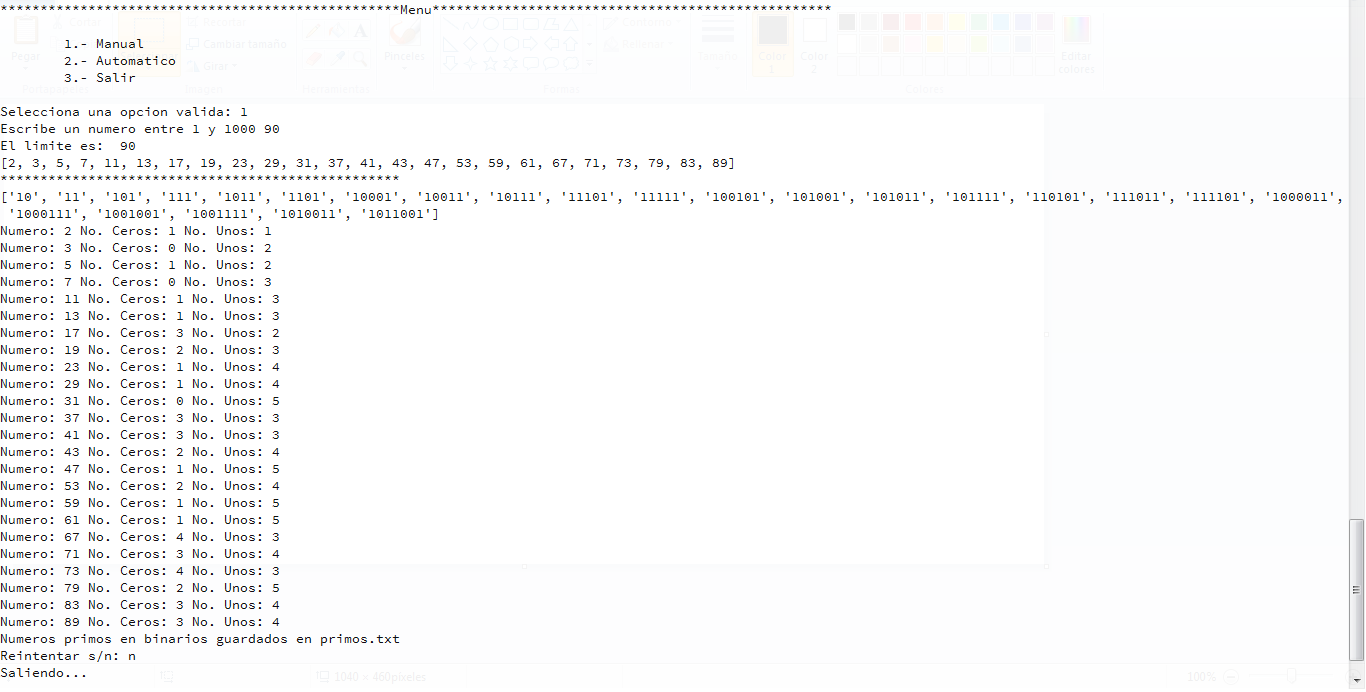
\includegraphics[width=\linewidth, height=10cm]{img/primos-manual.png}
				\caption{Modo automático n=90.}
				\label{fig:primos3}
			\end{center}
		\end{figure}
			\begin{figure}[H]
				\begin{center}
					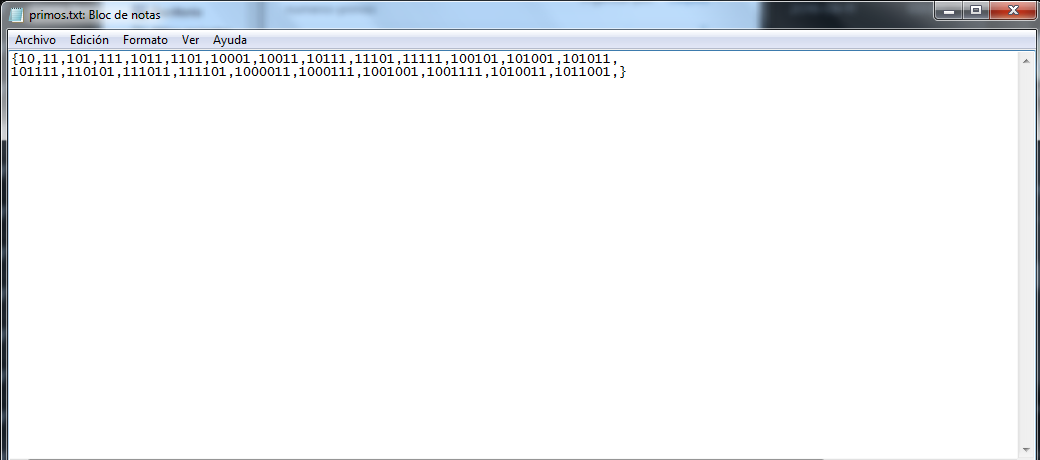
\includegraphics[width=\linewidth, height=7cm]{img/primos-manual-salida.png}
					\caption{Números primos en binario en el archivo.}
					\label{fig:primos4}
				\end{center}
			\end{figure}
	\begin{figure}[H]
		\begin{center}
			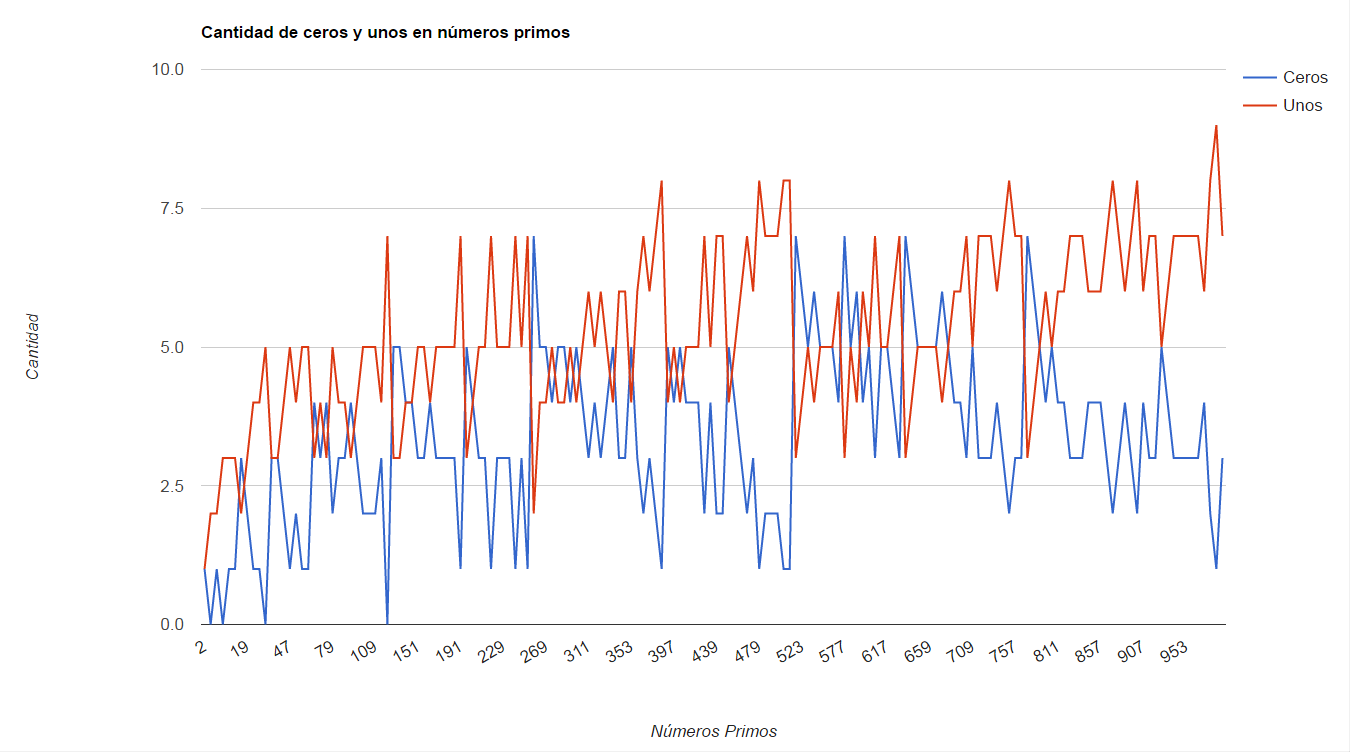
\includegraphics[width=\linewidth, height=7cm]{img/primos.png}
			\caption{Cantidad de ceros y unos encontrados entre 1 y 1000.}
			\label{fig:grafica}
		\end{center}
	\end{figure}
	\section{AFD Palabras con terminación 'ere'}
	\subsection{Descripción del problema}
	Desarrollar un autómata finito determinista capaz de encontrar las palabras con terminación 'ere' ya sea leyendo un archivo txt o en una linea de texto que el usuario ingresa, y que dichas palabras se muestren en pantalla y en el caso del archivo de texto imprimir la linea y el numero de palabra (por linea) en el que fue encontrada dicha palabra.
	Es importante señalar que todo aquello que no es un símbolo del alfabeto ingles, $ \sum =\lbrace a, b, ..., z, A, B, ..., Z \rbrace $, es tomado como un espacio. Además, debe tener una opción para visualizar el siguiente diagrama.
	\begin{figure}[H]
		\begin{center}
		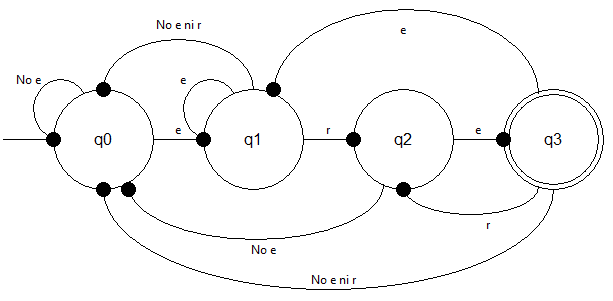
\includegraphics[width=14cm, height=7cm]{img/ere.png}
		\caption{Diagrama de transiciones del autómata 'ere'.}
		\label{fig:diagrama1}
		\end{center}
	\end{figure}
	\subsection{Código}
	El código fue realizado en Python 3.5.
	\\Archivo: main\_ere.py
	\begin{lstlisting}[language=Python]
	#main_ere.py
	# -*- coding: utf-8 -*-
	from __future__ import print_function
	from automata_ere import verificar_palabras
	from diagrama_ere import Diagrama
	
	separador = '*'*50
	
	def iniciar():
		continuar = True
		while continuar:
			opcion = imprimir_menu()
			if opcion == 1:
				entrada_consola()
			elif opcion == 2:
				entrada_archivo()
			elif opcion == 3:
				ver_diagrama()
			else:
				break
			print('*' * 100)
			opcion = input("Reintentar s/n: ")
			if opcion.lower() != 's':
				continuar = False
		
		print('Saliendo del programa...')
	
	def imprimir_menu():
		print("""Es importante mencionar que en este programa cualquier simbolo que no sea una letra en el alfabeto ingles separa una palabra de otra""")
		print('\n\n%sMenu%s' % (separador, separador))
		print("""
		1.- Entrada en consola
		2.- Ingresar nombre del archivo
		3.- Ver diagrama de estados
		4.- Salir
		""")
		try:
			opcion = int(input("Selecciona una opcion valida: "))
			return opcion
		except Exception as e:
			print('Error ', e)
			return 0
	
	def entrada_consola():
		texto = input("Escribe el texto: ")
		texto += ' '
		palabras_ere = []
		verificar_palabras(texto, palabras_ere)
		print('\n', palabras_ere)
	
	def entrada_archivo():
		archivo = input("Ingresa el nombre del archivo: ")
		try:
			archivo_abierto = open(archivo, 'r')
		except Exception as e:
			print('Error al abrir archivo: ', e)
			return 0
		
		linea_palabras = []
		num_linea = 1
		palabras_ere = []
		posiciones = []
		for linea in archivo_abierto:
			verificar_palabras(linea, palabras_ere, posiciones)
			linea_palabras.append({'Linea': num_linea, 'Palabras': palabras_ere, 'Posiciones': posiciones})
			num_linea += 1
			palabras_ere = []
			posiciones = []
		
		imprimir_archivo(linea_palabras)
		archivo_abierto.close()
	
	def imprimir_archivo(linea_palabras):
		print('\n\n')
		for elemento in linea_palabras:
			if len(elemento['Palabras']) > 0:
				print('Numero de linea: ', elemento['Linea'])
				i = 0
				for palabra in elemento['Palabras']:
					print('\tPalabra: %s No. Palabra: %s' % (palabra, elemento['Posiciones'][i]))
					i += 1
	
	def ver_diagrama():
		print('Mostrando diagrama del automata. Cierre la ventana para continuar')
		try:
			diagrama_ere = Diagrama()
			diagrama_ere.master.title('Diagrama del automata ere')
			diagrama_ere.mainloop()
		except Exception as e:
			print("Error", e)
	
	iniciar()
	\end{lstlisting}
	Archivo: automata\_ere.py
	\begin{lstlisting}[language=Python]
	#automata_ere.py
	# -*- coding: utf-8 -*-
	from __future__ import print_function
	
	def verificar_palabras(texto, palabras_ere, posiciones = []):
		palabra_aux = ''
		estado = 0
		num_palabra = 1
		for simbolo in texto:
			simbolo_aux = simbolo.lower()
			if simbolo ==  '\n':
				simbolo = '\\n'
			print('-> delta(q%s,%s)' % (estado, simbolo), end="\t")
			
			estado = automata(estado, simbolo_aux)
			
			if (ord(simbolo_aux) < 123 and ord(simbolo_aux) > 96):
				palabra_aux += simbolo
				if estado == 4:
					estado = 0
			else:
				if estado == 4:
					palabras_ere.append(palabra_aux)
					posiciones.append(num_palabra)
					estado = 0
				palabra_aux = ''
				if simbolo == ' ':
					num_palabra += 1
	
	def automata(estado, simbolo):
		if estado == 0:
			estado = estado_cero(simbolo)
		elif estado == 1:
			estado = estado_uno(simbolo)
		elif estado == 2:
			estado = estado_dos(simbolo)
		elif estado == 3:
			estado = estado_tres(simbolo)
		else:
			print('Simbolo extrano: ', simbolo)
		
		return estado
	
	def estado_cero(simbolo):
		if simbolo == 'e':
			return 1
		else:
			return 0
	
	def estado_uno(simbolo):
		if simbolo == 'r':
			return 2
		elif simbolo == 'e':
			return 1
		else:
			return 0
	
	def estado_dos(simbolo):
		if simbolo == 'e':
			return 3
		else:
			return 0
	
	def estado_tres(simbolo):
		if simbolo == 'r':
			return 2
		elif simbolo == 'e':
			return 1
		else:
			return 4
	\end{lstlisting}
	Archivo: diagrama\_ere.py
	\begin{lstlisting}[language=Python]
	#diagrama_ere.py
	# -*- coding: utf-8 -*-
	from __future__ import print_function
	import tkinter as tk
	
	class Diagrama(tk.Frame):
		def __init__(self, master=None):
			super().__init__(master, background='white')
			self.pack(fill=tk.BOTH, expand=tk.YES)
			self.dibujarDiagrama()
			self.centrarVentana()
	
		def dibujarDiagrama(self):
			canvas = tk.Canvas(self, bg='white')
			datos = {}
			datos['coordenadas'] = [100, 100, 200, 200]
			datos['canvas'] = canvas
			self.circulos_flechas(datos)
			
			self.crear_arco(canvas, [150, 50, 300, 150])
			canvas.create_text(150+75, 50-15, text='No e ni r')
			self.crear_arco(canvas, [320, 20, 585, 190])
			canvas.create_text(320+130, 50-10, text='e')
			# reflexiva
			extra = {'start': 30, 'extend': 235}
			self.crear_arco(canvas, [80, 90, 135, 150], extra)
			canvas.create_text(80-5, 90, text='No e')
			self.crear_arco(canvas, [230, 90, 285, 150], extra)
			canvas.create_text(230, 90, text='e')
			
			#de cabeza
			extra = {'start': 0, 'extend': -180}
			self.crear_arco(canvas, [150, 100, 600, 300], extra)
			canvas.create_text(600-220, 300-10, text='No e ni r')
			self.crear_arco(canvas, [175, 140, 430, 250], extra)
			canvas.create_text(430-120, 300-40, text='No e')
			self.crear_arco(canvas, [450, 170, 585, 225], extra)
			canvas.create_text(585-50, 225+10, text='r')
			
			canvas.pack(fill=tk.BOTH, expand=1)
		
		def circulos_flechas(self, arg):
			coordenadas = arg['coordenadas']
			canvas = arg['canvas']
			for x in range(4):
				self.escribirTexto(canvas, x, coordenadas)
				self.dibujarCirculo(canvas, coordenadas)
				self.dibujarFlecha(canvas, [coordenadas[0]-50, 150, coordenadas[2]-100, 150])
				coordenadas[0] += 150
				coordenadas[2] += 150
			
			self.dibujarCirculo(canvas, [coordenadas[0]-150+5, 105, coordenadas[2]-155, 195]) # circulo interior
		
		def escribirTexto(self, canvas, x, coordenadas):
			text = ''
			text_flecha =''
			if x == 0:
				text = 'q%s' % x
				text_flecha = ''
			elif x == 1:
				text = 'q%s' % x
				text_flecha = 'e'
			elif x == 2:
				text = 'q%s' % x
				text_flecha = 'r'
			elif x == 3:
				text = 'q%s' % x
				text_flecha = 'e'
			else:
				print('otro')
		
			canvas.create_text(coordenadas[0]+50, coordenadas[1]+50, font=('15'), text=text)
			canvas.create_text(coordenadas[0]-25, coordenadas[1]+40, text=text_flecha)
		
		def dibujarCirculo(self, canvas, coordenadas):
			circulo = canvas.create_oval(coordenadas)
		
		def dibujarFlecha(self, canvas, coordenadas):
			linea = canvas.create_line(coordenadas)
			canvas.create_oval(coordenadas[2]-7, coordenadas[1]-7, coordenadas[2]+7,coordenadas[1]+7, fill = 'black')
		
		def crear_arco(self, canvas, coordenadas, extra=None):
			if extra != None:
				arco = canvas.create_arc(coordenadas, start=extra['start'], extent=extra['extend'], style='arc')
				if extra['extend'] == -180:
					canvas.create_oval(coordenadas[0]-7, 100+100-7, coordenadas[0]+7, 100+100+7, fill = 'black')
			else:
				arco = canvas.create_arc(coordenadas, start=0, extent=180, style='arc')
				canvas.create_oval(coordenadas[0]-7, 100-7, coordenadas[0]+7, 100+7, fill = 'black')
		
		def centrarVentana(self):
			ancho, altura = 700, 350
			ancho_pantalla = self.winfo_screenwidth()
			altura_pantalla = self.winfo_screenheight()
			posicion_x = (ancho_pantalla - ancho)/2
			posicion_y = (altura_pantalla - altura)/2
			self.master.geometry('%dx%d+%d+%d' % (ancho, altura, posicion_x, posicion_y))
	
	\end{lstlisting}
	\subsection{Pruebas}
	Pruebas de las opciones del menú.
	\\
	{\large Modo de consola.}
	\begin{figure}[H]
		\begin{center}
			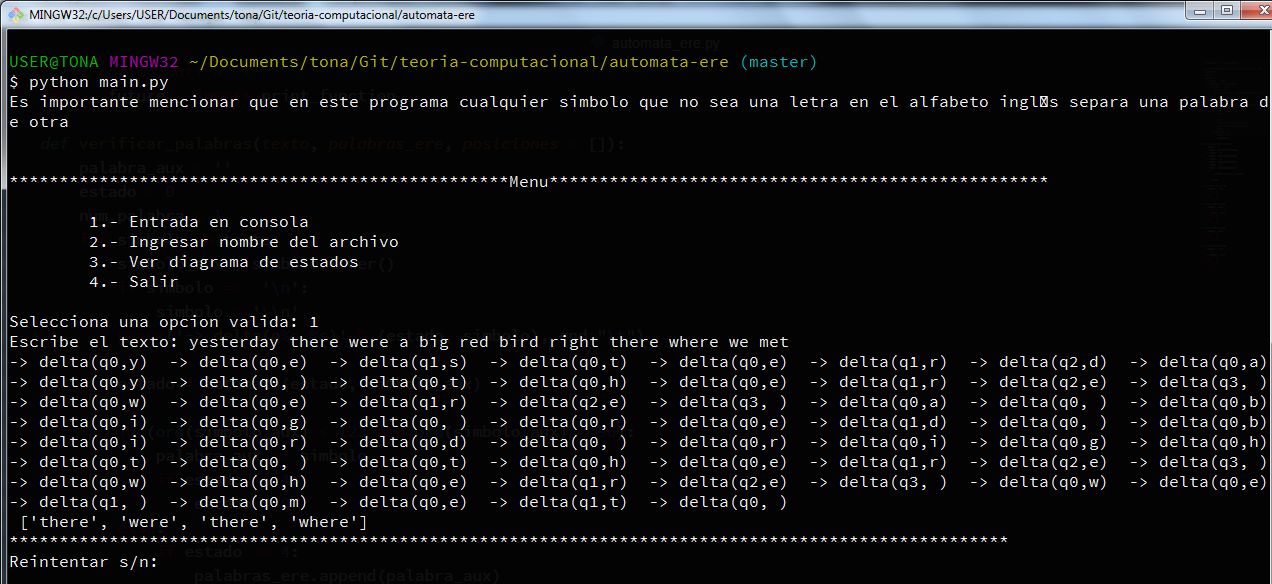
\includegraphics[width=\linewidth, height=6cm]{img/ere-manual.png}
			\caption{Historia del autómata y las palabras con terminación 'ere'.}
			\label{fig:ere1}
		\end{center}
	\end{figure}
	{\large Modo archivo.}
	\begin{figure}[H]
		\begin{center}
			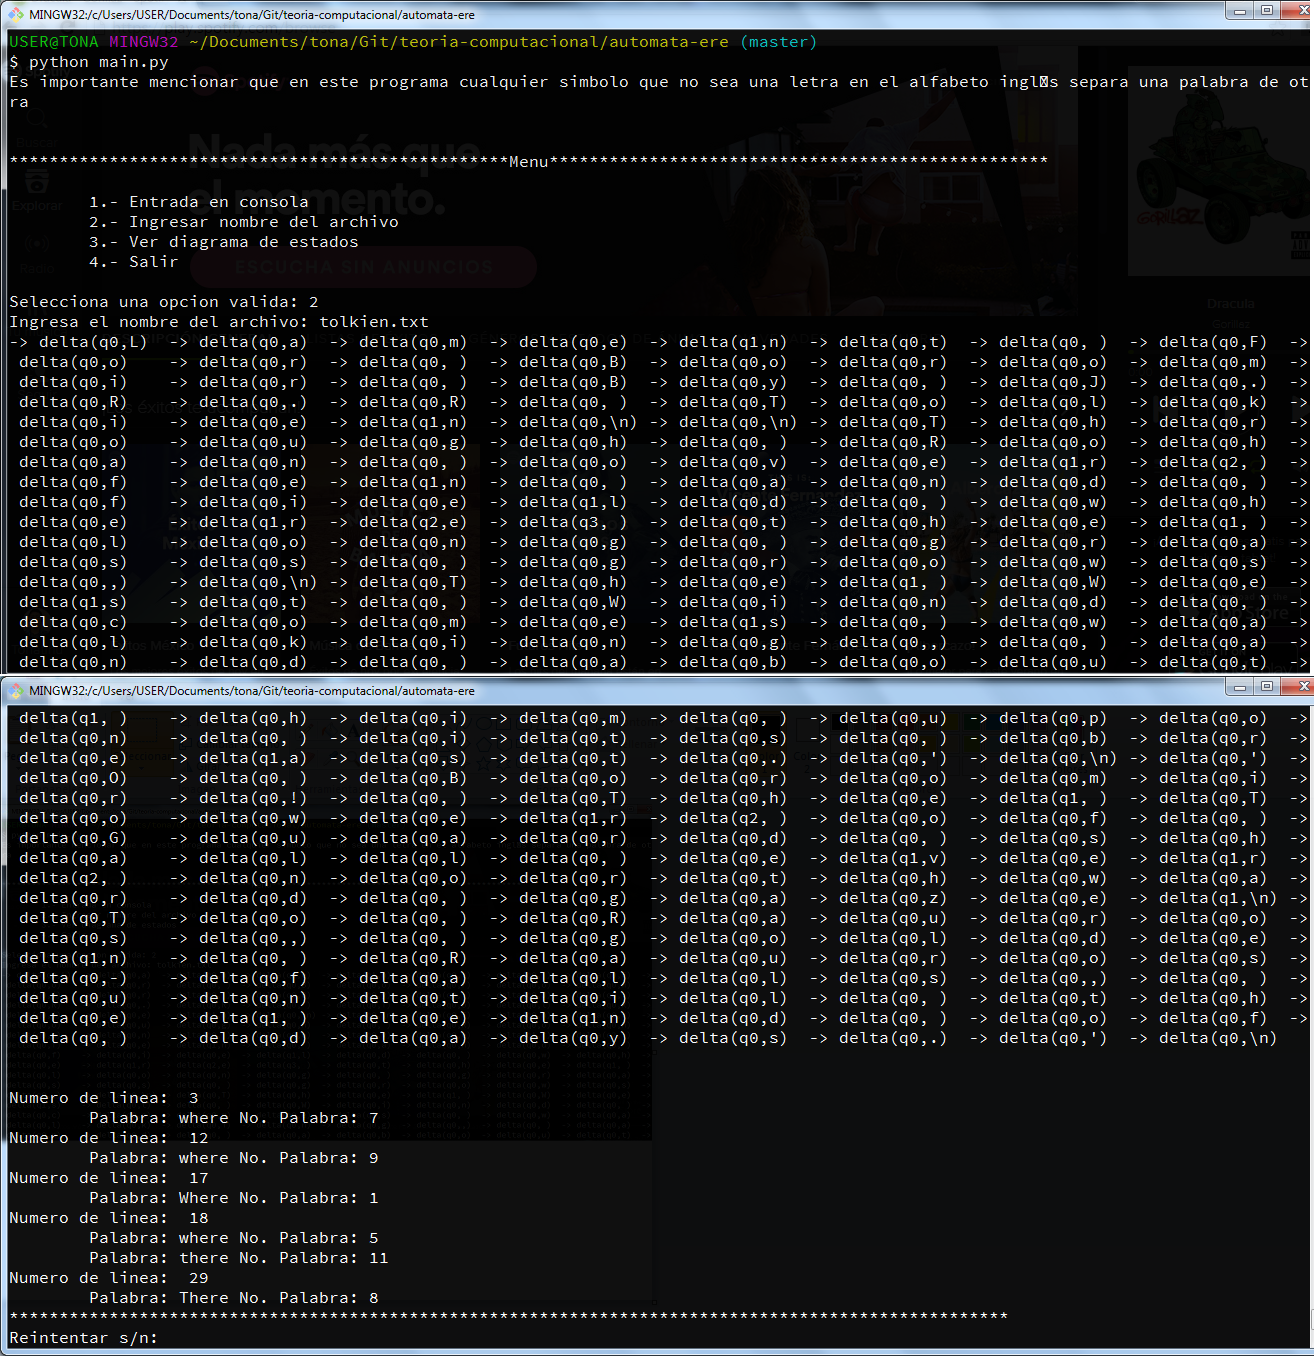
\includegraphics[width=\linewidth, height=20cm]{img/ere-automatico.png}
			\caption{Parte de la historia del autómata y las palabras con terminación 'ere'.}
			\label{fig:ere2}
		\end{center}
	\end{figure}
	{\large Diagrama.}
	\begin{figure}[H]
		\begin{center}
			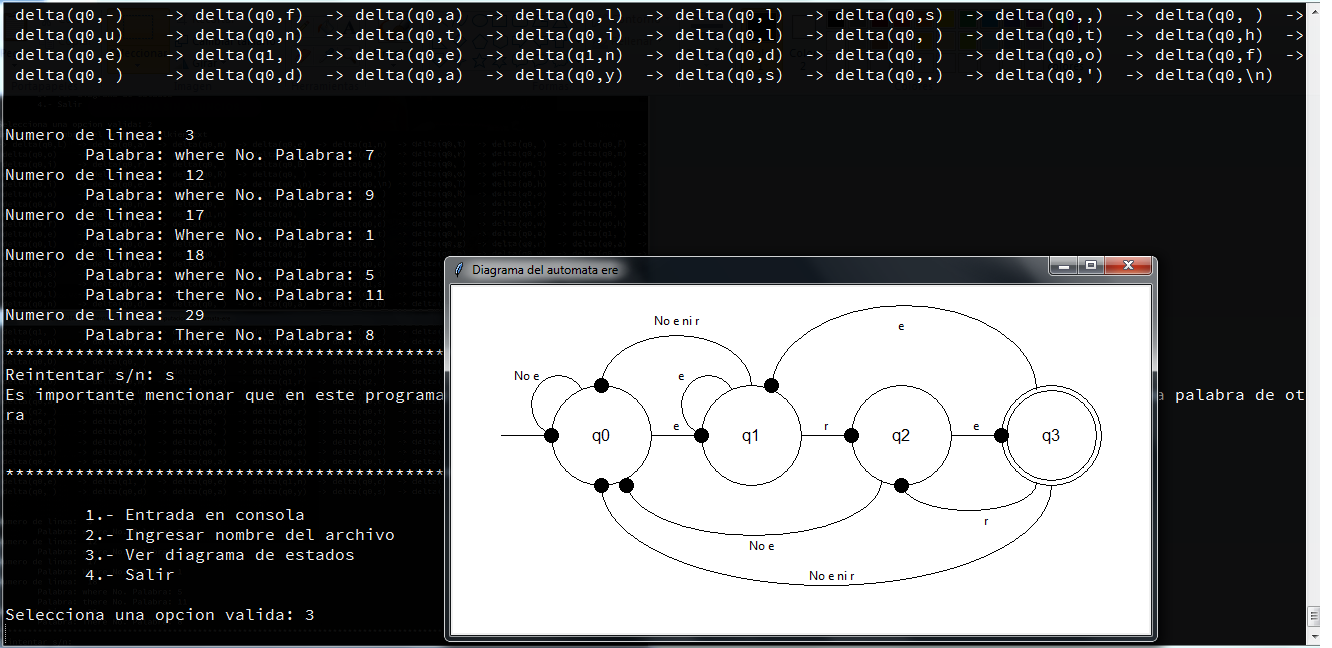
\includegraphics[width=\linewidth, height=9cm]{img/diagrama-ere.png}
			\caption{Diagrama de transiciones del autómata 'ere'.}
			\label{fig:ere3}
		\end{center}
	\end{figure}
	\section{AFD Paridad en números binarios}
	\subsection{Descripción del problema}
	Diseñar y programar un autómata finito determinista que acepte el lenguaje:
	\[ L = \lbrace w \mid w \text{ tiene un número par de ceros y un numero par de unos} \rbrace \text{\cite{LIBRO}}\] 
	Es decir, los números binarios de entrada se generan de manera automática (cadena de longitud $n \mid 1\leq n \leq 1000$) o manual y después se imprime si es una cadena valida o no y en ambos casos imprimir su historia. Ademas, mostrar el siguiente diagrama.
	\begin{figure}[H]
		\begin{center}
			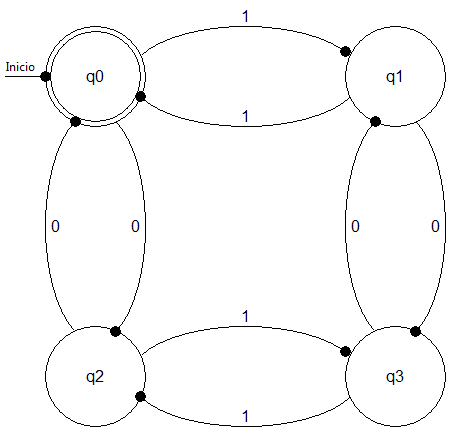
\includegraphics[width=7cm, height=7cm]{img/paridad.png}
			\caption{Diagrama de transiciones del autómata. \cite{LIBRO}}
			\label{fig:diagrama2}
		\end{center}
	\end{figure}
	\subsection{Código}
	El código fue realizado en Python 3.5.
	\\Archivo: main\_paridad.py
	\begin{lstlisting}[language=Python]
	#main_paridad.py
	# -*- coding: utf-8 -*-
	from __future__ import print_function
	from automata_paridad import ejecutar_automata
	from diagrama_paridad import Diagrama
	import random
	
	separador = '*' * 50
	def iniciar():
		continuar = True
		while continuar:
			opcion = imprimir_menu()
			if opcion == 1:
				ejecutar_manual()
			elif opcion == 2:
				ejecutar_random()
			elif opcion == 3:
				ver_diagrama()
			else:
				break
			print('\n', separador)
			opcion = input("Reintentar s/n: ")
			if opcion.lower() != 's':
				continuar = False
		
		print('Saliendo del programa...')
	
	def imprimir_menu():
		print('\n\n%sMenu%s' % (separador, separador))
		print("""
		1.- Entrada en consola (Manual)
		2.- Numero aleatorio (automatico)
		3.- Ver diagrama de transiciones
		4.- Salir
		""")
		try:
			opcion = int(input("Selecciona una opcion valida: "))
			return opcion
		except Exception as e:
			print('Error ', e)
			return 0
	
	def ejecutar_random():
		i = 0
		longitud_random = random.randint(1, 1000)
		numero_binario = ''
		while i < longitud_random:
			numero_binario += random.choice(['0', '1'])
			i += 1
		
		print("El numero aleatorio es: ", numero_binario)
		provar_paridad(numero_binario)
	
	def ejecutar_manual():
		numero_binario = input("Escribe un numero binario: ")
		provar_paridad(numero_binario)
	
	def provar_paridad(numero_binario):
		resultado = ejecutar_automata(numero_binario)
		print('\n')
		if resultado:
			print('El numero %s, es valido' % numero_binario)
		else:
			print('El numero: %s, no es valido' % numero_binario)
	
	def ver_diagrama():
		print('Mostrando diagrama del automata. Cierre la ventana para continuar')
		try:
			diagrama_paridad = Diagrama()
			diagrama_paridad.master.title('Diagrama del automata paridad')
			diagrama_paridad.mainloop()
		except Exception as e:
			print("Error", e)
	
	iniciar()
	\end{lstlisting}
	Archivo: automata\_paridad.py
	\begin{lstlisting}[language=Python]
	#automata_paridad.py
	def ejecutar_automata(cadena):
		estado = 0
		for simbolo in cadena:
			print('-> delta(q%s,%s)' % (estado, simbolo), end="\t")
			estado = automata(estado, simbolo)
			if estado == -1:
				break
		if estado == 0:
			print('-> delta(q%s, )' % estado, end="\t")
			return True
		return False
	
	def automata(estado, simbolo):
		if estado == 0:
			estado = estado_cero(simbolo)
		elif estado == 1:
			estado = estado_uno(simbolo)
		elif estado == 2:
			estado = estado_dos(simbolo)
		elif estado == 3:
			estado = estado_tres(simbolo)
		else:
			print('Simbolo extrano ', simbolo)
			return -1
		return estado
	
	def estado_cero(simbolo):
		if simbolo == '0':
			return 2
		elif simbolo == '1':
			return 1
		else:
			return -1
	
	def estado_uno(simbolo):
		if simbolo == '0':
			return 3
		elif simbolo == '1':
			return 0
		else:
			return -1
		
	def estado_dos(simbolo):
		if simbolo == '0':
			return 0
		elif simbolo == '1':
			return 3
		else:
			return -1
	
	def estado_tres(simbolo):
		if simbolo == '0':
			return 1
		elif simbolo == '1':
			return 2
		else:
			return -1
	\end{lstlisting}
	Archivo: diagrama\_paridad.py
	\begin{lstlisting}[language=Python]
	#diagrama_paridad.py
	# -*- coding: utf-8 -*-
	from __future__ import print_function
	import tkinter as tk
	
	class Diagrama(tk.Frame):
		def __init__(self, master=None):
			super().__init__(master, background='white')
			self.pack(fill=tk.BOTH, expand=tk.YES)
			self.canvas = tk.Canvas(self, bg='white')
			self.canvas.pack(fill=tk.BOTH, expand=1)
			self.dibujarDiagrama()
			self.centrarVentana()
		
		def dibujarDiagrama(self):
			self.dibujarFlecha([10, 100, 50, 100])
			self.dibujarCirculo([55, 55, 145, 145])
			for x in range(4):
				if x == 0:
					coordenadas = [50, 50, 150, 150]
					text_circulo = 'q%s' % x
					self.dibujarFlechaHorizontal(coordenadas[:])
					self.dibujarFlechaVertical(coordenadas[:])
				elif x == 1:
					coordenadas = [350, 50, 450, 150]
					text_circulo = 'q%s' % x
					self.dibujarFlechaVertical(coordenadas[:])
				elif x == 2:
					coordenadas = [50, 350, 150, 450]
					text_circulo = 'q%s' % x
					self.dibujarFlechaHorizontal(coordenadas[:])
				elif x == 3:
					coordenadas = [350, 350, 450, 450]
					text_circulo = 'q%s' % x
				
				else:
					print('Na')
				
				self.dibujarCirculo(coordenadas)
				self.canvas.create_text(coordenadas[0]+50, coordenadas[1]+50, font=('15'), text=text_circulo)
			
		def dibujarCirculo(self, arg):
			circulo = self.canvas.create_oval(arg)
		
		def dibujarFlechaHorizontal(self, coordenadas):
			coordenadas[0] += 85
			coordenadas[2] += 215
			x = ((coordenadas[2] - coordenadas[0])/2) + coordenadas[0]
			
			self.canvas.create_text(x, coordenadas[1]-10, font=('15'), text='1')
			self.canvas.create_text(x, coordenadas[3]-10, font=('15'), text='1')
			
			self.canvas.create_arc(coordenadas, start=25, extent=130, style='arc')
			self.canvas.create_arc(coordenadas, start=-25, extent=-130, style='arc')
			
			self.canvas.create_oval(coordenadas[2]-5-15, coordenadas[1]-5+25, coordenadas[2]+5-15, coordenadas[1]+5+25, fill = 'black')
			self.canvas.create_oval(coordenadas[0]-5+10, coordenadas[3]-5-30, coordenadas[0]+5+10, coordenadas[3]+5-30, fill = 'black')
		
		def dibujarFlechaVertical(self, coordenadas):
			coordenadas[1] += 85
			coordenadas[3] += 215
			
			y = ((coordenadas[3] - coordenadas[1])/2) + coordenadas[1]
			
			self.canvas.create_text(coordenadas[0]+10, y, font=('15'), text='0')
			self.canvas.create_text(coordenadas[2]-10, y, font=('15'), text='0')
			
			self.canvas.create_arc(coordenadas, start=-65, extent=130, style='arc')
			self.canvas.create_arc(coordenadas, start=115, extent=130, style='arc')
			
			self.canvas.create_oval(coordenadas[0]-5+30, coordenadas[3]-5-220, coordenadas[0]+5+30, coordenadas[3]+5-220, fill = 'black')
			self.canvas.create_oval(coordenadas[2]-5-30, coordenadas[1]-5+220, coordenadas[2]+5-30, coordenadas[1]+5+220, fill = 'black')
		
		def dibujarFlecha(self, coordenadas):
			linea = self.canvas.create_line(coordenadas)
			self.canvas.create_text(coordenadas[0]+15, coordenadas[1]-10, text='Inicio')
			self.canvas.create_oval(coordenadas[2]-5, coordenadas[1]-5, coordenadas[2]+5,coordenadas[1]+5, fill = 'black')
		
		def centrarVentana(self):
			ancho, altura = 500, 500
			ancho_pantalla = self.winfo_screenwidth()
			altura_pantalla = self.winfo_screenheight()
			posicion_x = (ancho_pantalla - ancho)/2
			posicion_y = (altura_pantalla - altura)/2
			self.master.geometry('%dx%d+%d+%d' % (ancho, altura, posicion_x, posicion_y))
	\end{lstlisting}
	\newpage
	\subsection{Pruebas}
	Pruebas de las opciones del menú.
	\\{\large Modo manual.}
	\begin{figure}[H]
		\begin{center}
			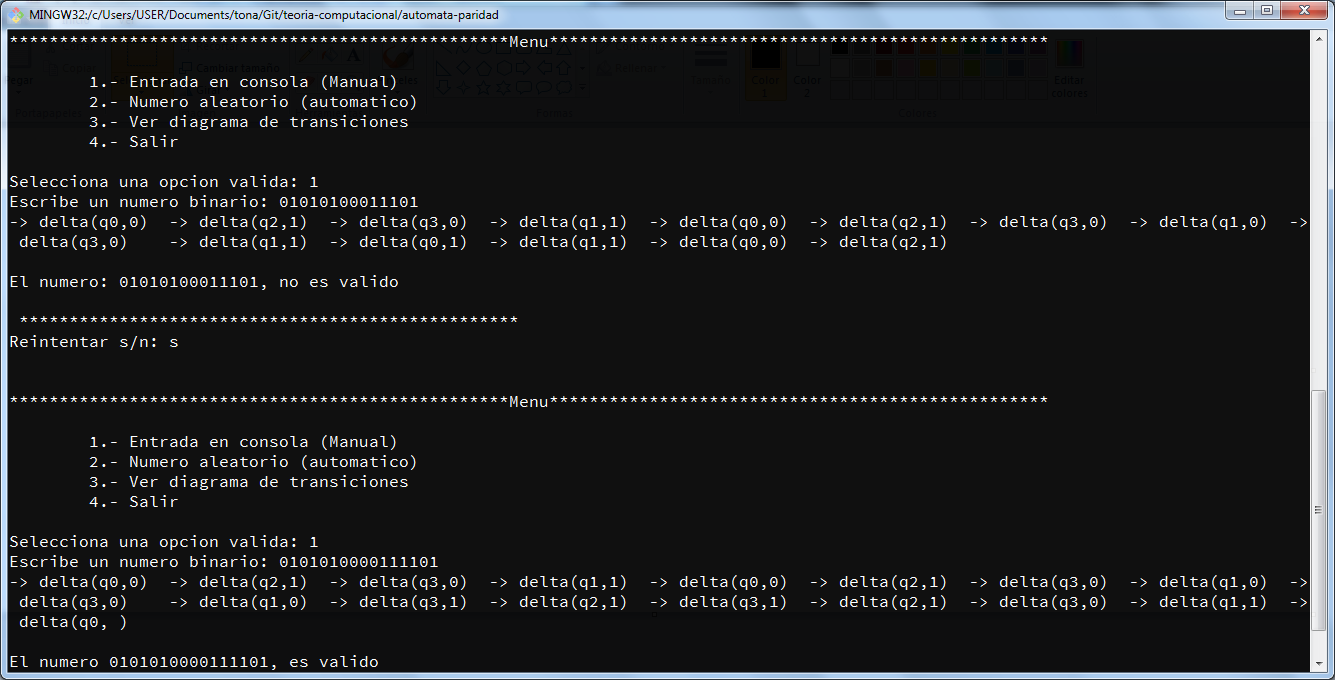
\includegraphics[width=\linewidth, height=8cm]{img/manual-paridad.png}
			\caption{Historia del autómata}
			\label{fig:paridad2}
		\end{center}
	\end{figure}
	{\large Modo automático.}
	\begin{figure}[H]
		\begin{center}
			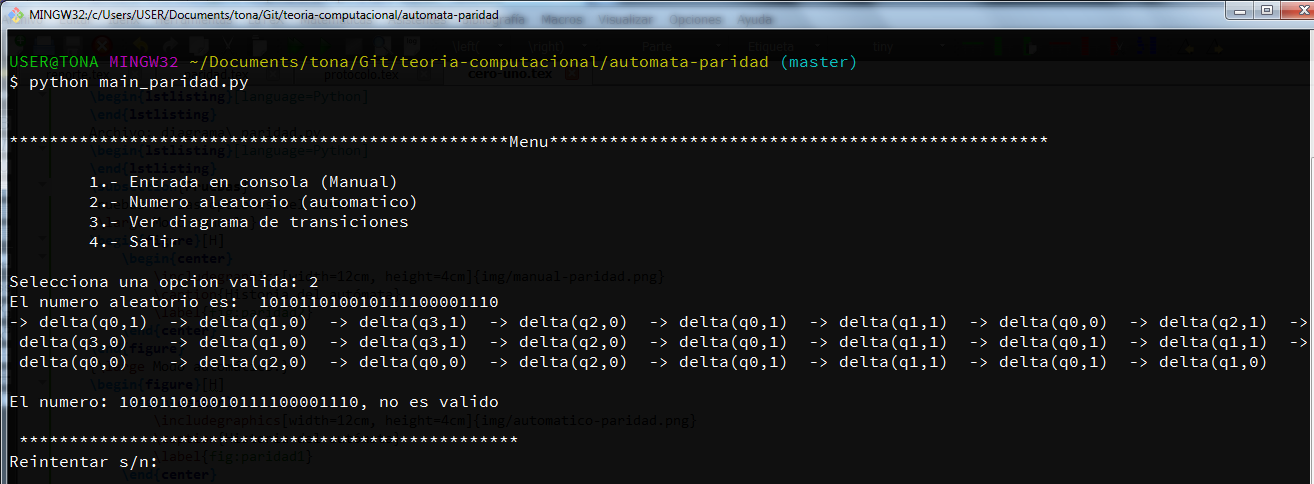
\includegraphics[width=\linewidth, height=8cm]{img/automatico-paridad.png}
			\caption{Historia del autómata}
			\label{fig:paridad1}
		\end{center}
	\end{figure}
	{\large Diagrama.}
	\begin{figure}[H]
		\begin{center}
			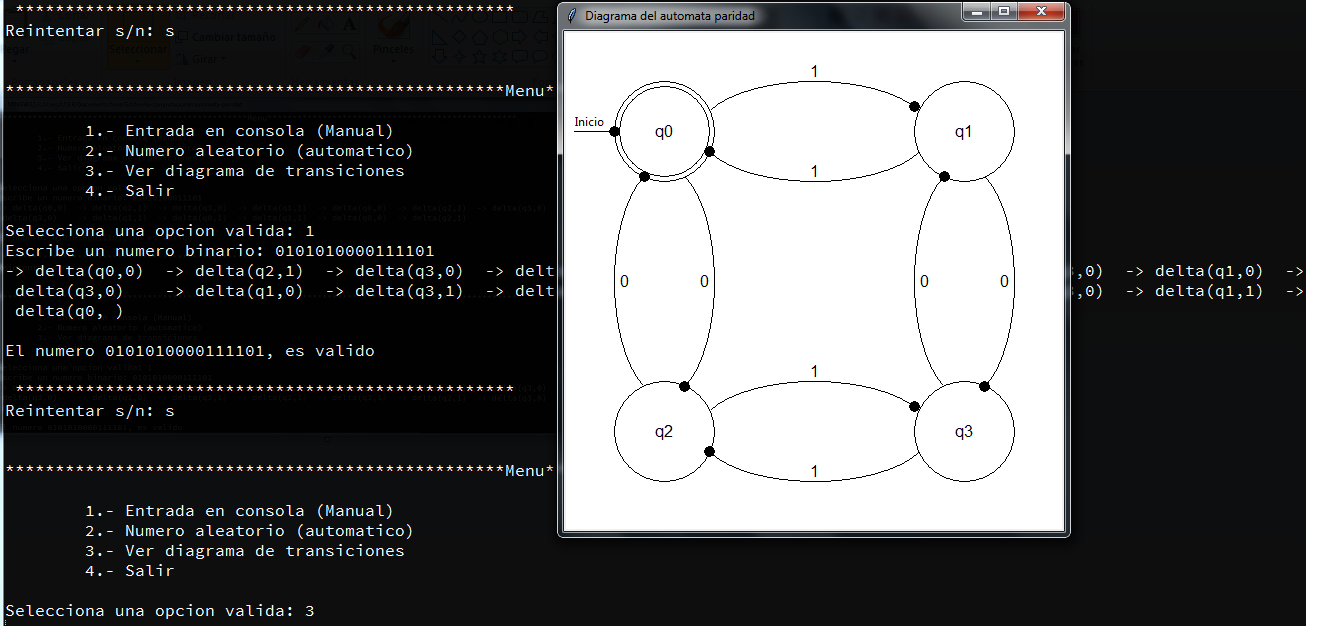
\includegraphics[width=\linewidth, height=8cm]{img/diagrama-paridad.png}
			\caption{Diagrama de transiciones del autómata}
			\label{fig:paridad3}
		\end{center}
	\end{figure}
	\section{Protocolo de transmisión}
	\subsection{Descripción del problema}
	Desarrollar un programa que genere 50 cadenas de 32 caracteres que sean guardadas en un archivo, para después ser evaluadas por un autómata, en este caso el de paridad binaria y guardar las cadenas binarias validas en otro archivo, siguiendo el siguiente diagrama.
	\begin{figure}[H]
		\begin{center}
			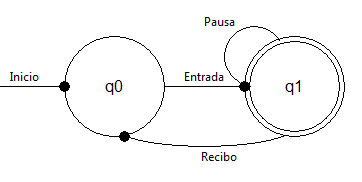
\includegraphics[width=10cm, height=5cm]{img/protocolo.png}
			\caption{Diagrama de transiciones del autómata. \cite{WEB}}
			\label{fig:diagrama3}
		\end{center}
	\end{figure}
	\subsection{Código}
	El código fue realizado en Python 3.5.
	\subsection{Pruebas}
	Pruebas de las opciones del menú.
	{\large Modo automático.}
	\begin{figure}[H]
		\begin{center}
			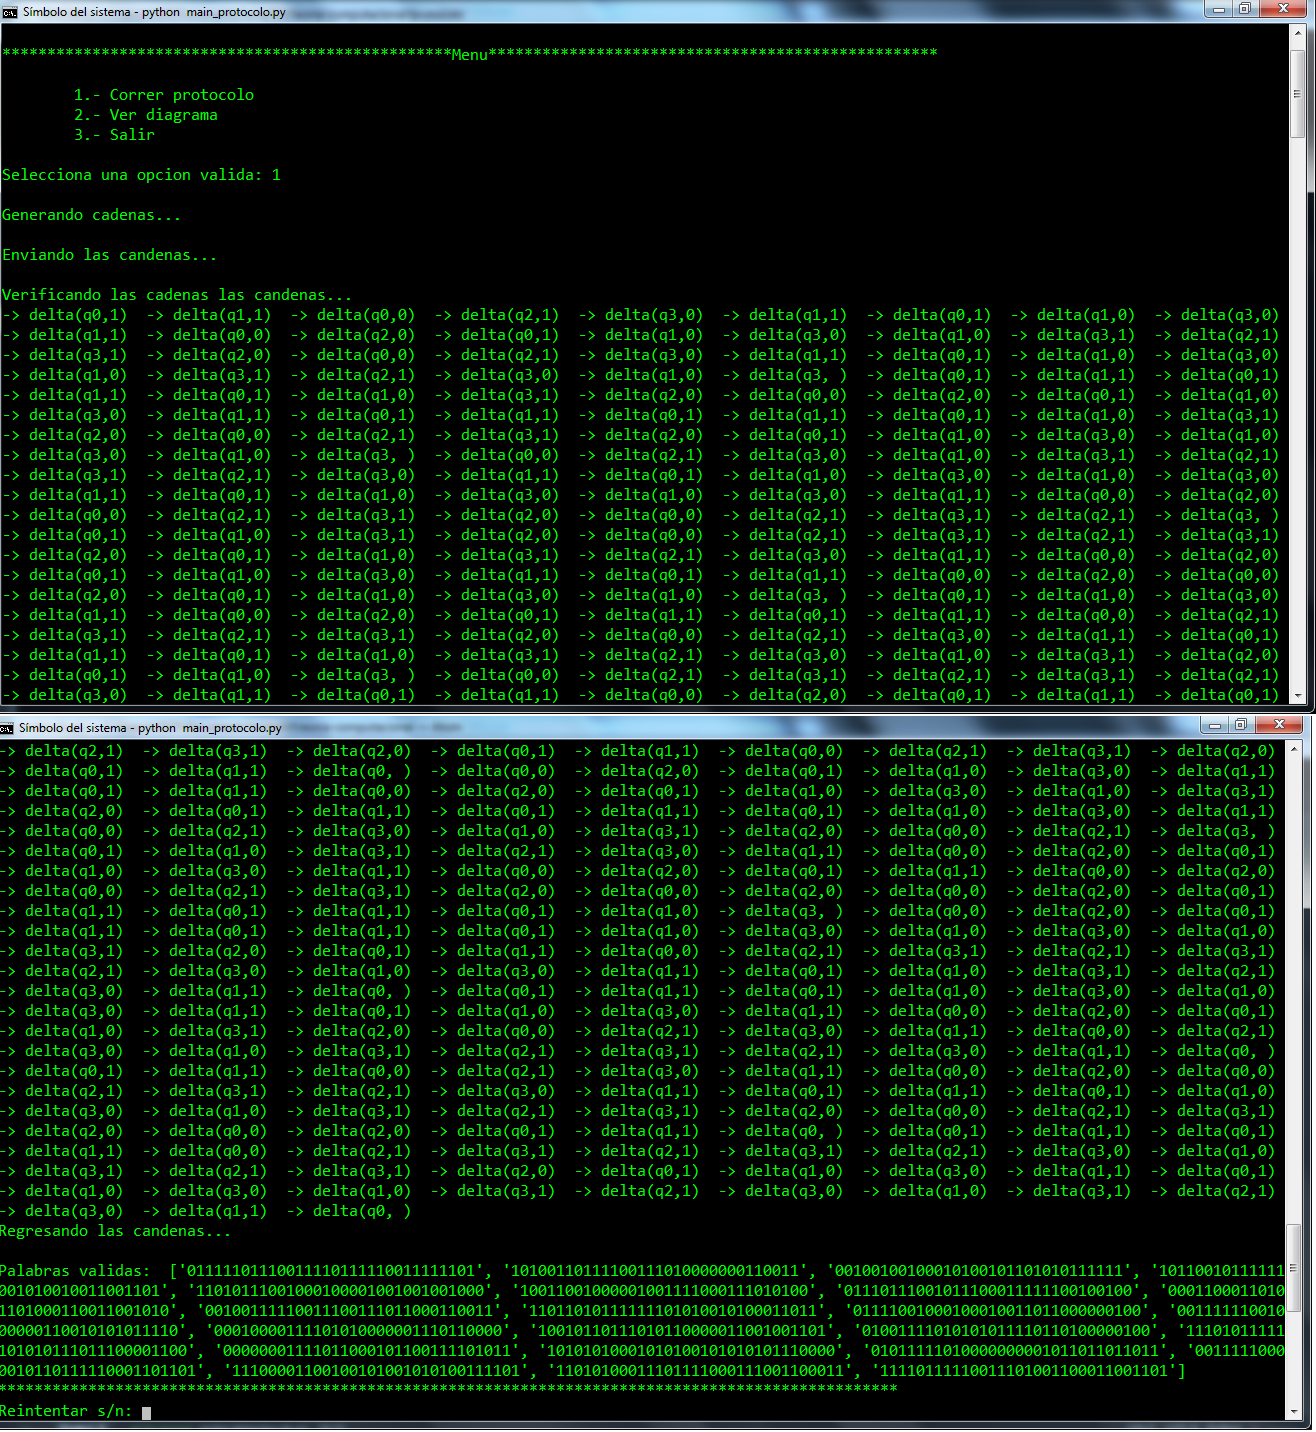
\includegraphics[width=10cm, height=5cm]{img/protocolo-automata.png}
			\caption{Historia del protocolo. \cite{WEB}}
			\label{fig:protocolo1}
		\end{center}
	\end{figure}
	\begin{figure}[H]
		\begin{center}
			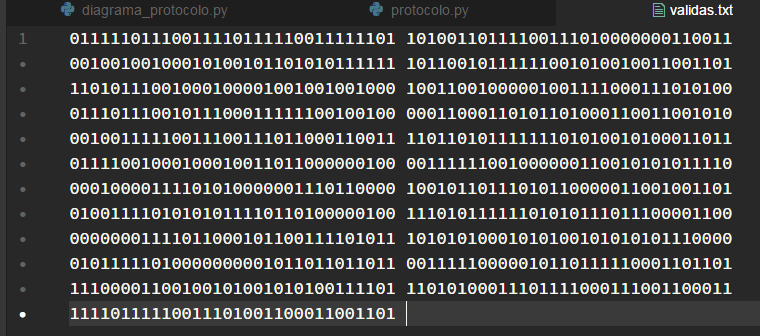
\includegraphics[width=10cm, height=5cm]{img/protocolo-salida.png}
			\caption{Palabras validas. \cite{WEB}}
			\label{fig:protocolo2}
		\end{center}
	\end{figure}
	{\large Diagrama.}
	\begin{figure}[H]
		\begin{center}
			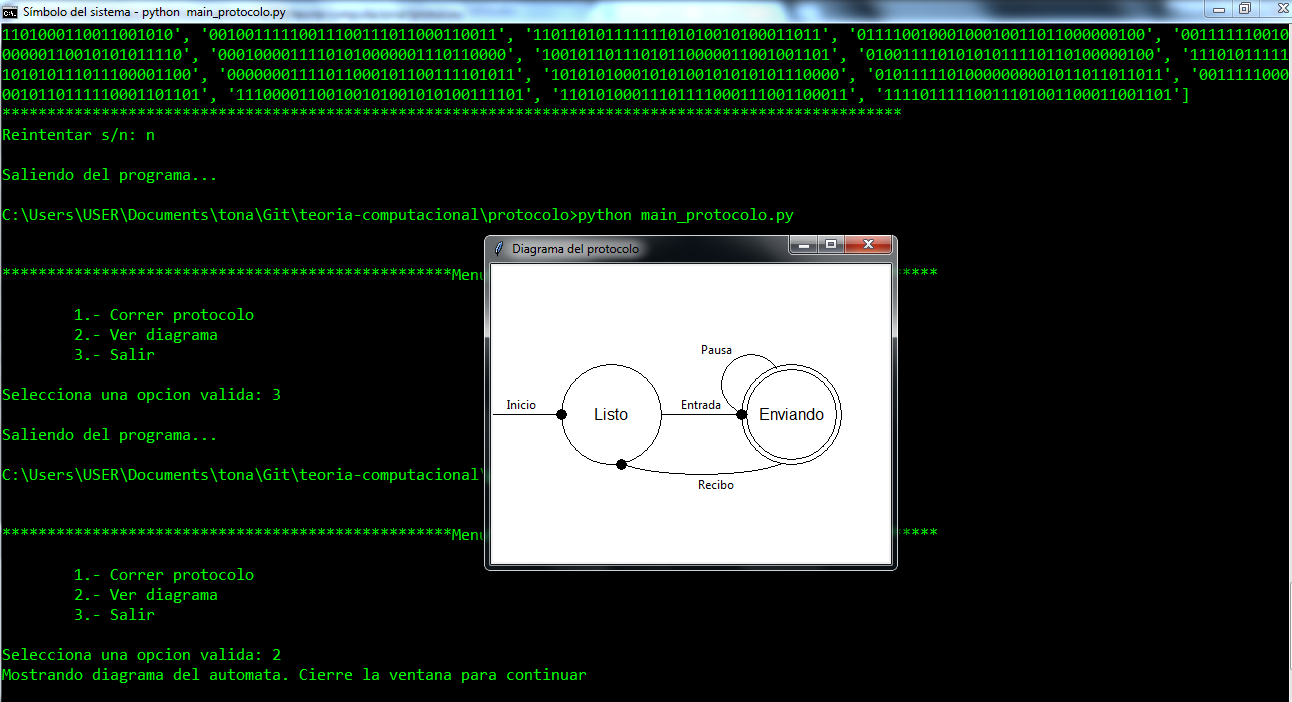
\includegraphics[width=10cm, height=5cm]{img/protocolo-diagrama.png}
			\caption{Diagrama de transiciones del autómata.}
			\label{fig:protocolo3}
		\end{center}
	\end{figure}
	\section{AFND Números binarios con terminación '01'}
	\subsection{Descripción del problema}
	Desarrollar un autómata finito no determinista, que acepte todas y sólo las cadenas formadas por ceros y unos que terminan en 01. Asimismo, imprimir la tabla de transiciones (historia) y que la entrada de cadenas sea de forma manual o automática, la cadena automática debe de tener una longitud $n \mid 1  \leq n \leq 1000$. Y que contenga la opción de mostrar el siguiente diagrama.
	\begin{figure}[ht]
		\begin{center}
			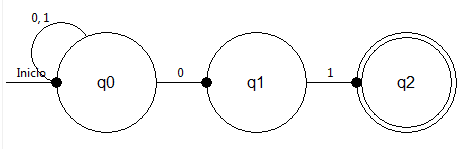
\includegraphics[width=12cm, height=4cm]{img/cero-uno.png}
			\caption{Diagrama de transiciones del autómata. \cite{LIBRO}}
			\label{fig:diagrama4}
		\end{center}
	\end{figure}
	
	\subsection{Código}
	El código fue realizado en Python 3.5.
	\subsection{Pruebas}
	Pruebas de las opciones del menú.
	{\large Modo automático.}
	{\large Modo manual.}
	{\large Diagrama.}
	
	\bibliography{bibliografia} 
	\bibliographystyle{ieeetr}
\end{document}